% !TEX TS-program = pdflatex
% !TEX encoding = UTF-8 Unicode

\documentclass{article}
\usepackage[utf8]{inputenc}

\usepackage{graphicx} % support the \includegraphics command and options
\usepackage[parfill]{parskip} % Activate to begin paragraphs with an empty line rather than an indent
\usepackage{array} % for better arrays (eg matrices) in maths
\usepackage{paralist} % very flexible & customisable lists (eg. enumerate/itemize, etc.)
\usepackage{verbatim} % adds environment for commenting out blocks of text & for better verbatim
\usepackage{subfig} % make it possible to include more than one captioned figure/table in a single float



\title{DD1346 - Javaprojekt - Projektplan}
\author{Carl Svensson, F-10 \\ Carl Aronsson, F-10}
\begin{document}
%\date{}
\maketitle

\section{Översikt}

Chatklienten är strukturerad enligt MVC-mönstret. View-delen består av ett flertal klasses som representerar fönster och paneler.
Controller-delen är delad i två klasser, en klass som sköter generella saker för hela programmet och en klass som har ett objekt för varje chatt.
Model-delen har en klass för inställningar och tillstånd som gäller hela programmet och en klass som har ett objekt per chatt.

\section{Klasser}

\subsection{View}
\begin{description}
  \item[ProgramView] \hfill \\
  Huvuprogrammet, innehåller en menyrad, en ruta med flikar innehållandes instanser av ChatView samt en MessageComposerView.
  \item[ChatView] \hfill \\
  Representerar en chat. Visar en lista med chattens deltagare och alla meddelanden som skrivits.
  \item[MessageComposerView] \hfill \\
  Textredigeraren, innehåller en textruta samt alternativ för att formatera texten och välja kryptering.
  \item[AboutBoxView] \hfill \\
  Dialogruta som öppnas när man trycker på Help $\rightarrow$ About. Visar vilka som tillverkat programmet samt versionsinformation.
  \item[SettingsView] \hfill \\
  Ger användaren möjlighet att visa och redigera inställningar så som lyssningsport och namn.
  \item[FileTransferStartView] \hfill \\
  Dialog för att påbörja en filöverföring. Låter användaren välja en fil och skriva ett meddelande.
  \item[FileTransferRequestView] \hfill \\
  Dialogruta för inkommande filöverföringsförfrågan. Visar filnamnet och meddelandet samt låter användaren välja om den ska ta emot den.
  \item[FileTransferView] \hfill \\
  Dialogruta som visar status på en pågående filöverföring.
  \item[NewChatView] \hfill \\
  Dialogruta för att skapa en ny chatt. Låter användaren bestämma om den ska ansluta till en annan chat eller skapa en gruppchatt.
\end{description}

\subsection{Controller}
\begin{description}
  \item[ProgramCtrl] \hfill \\
  Programkontrollen, sköter globala inställningar, öppnande och stängande av dialogrutor och skapande av nya chattar.
\item[ProgramCtrl] \hfill \\
  Chattkontrollen, sköter en chattsession. Tar emot och skickar meddelanden till en eller flera klienter.
\end{description}

\subsection{Model}
\begin{description}
  \item[ProgramSettingsMdl] \hfill \\
  Lagrar inställningar för programmet så som port och namn. Låter även programmet spara dessa och läsa in dem från en fil.
\item[ChatMdll] \hfill \\
  Chatmodell, innehåller anslutningar och användare i en chatt. Lagrar även meddelandeinställningar i ett MessageSetting-objekt. Ansvarar även för initiering av filöverföring samt kryptering.
\item[MessageSettings] \hfill \\
  Meddelandeinställningar, lagrar inställningar som skickar till MessageComposerView när chatten blir den aktiva. Detta eftersom det bara finns ett sådant objekt men flera chattar.
\end{description}

\pagebreak

\section{UML}

Nedan visas programmets UML-klassdiagram med klassernas viktigaste funktioner samt hur kompositionen ser ut.

\begin{figure}[h!tb]
  %\caption{Programmets UML-klassdiagram.}
  \centering
  \makebox[\textwidth][c]{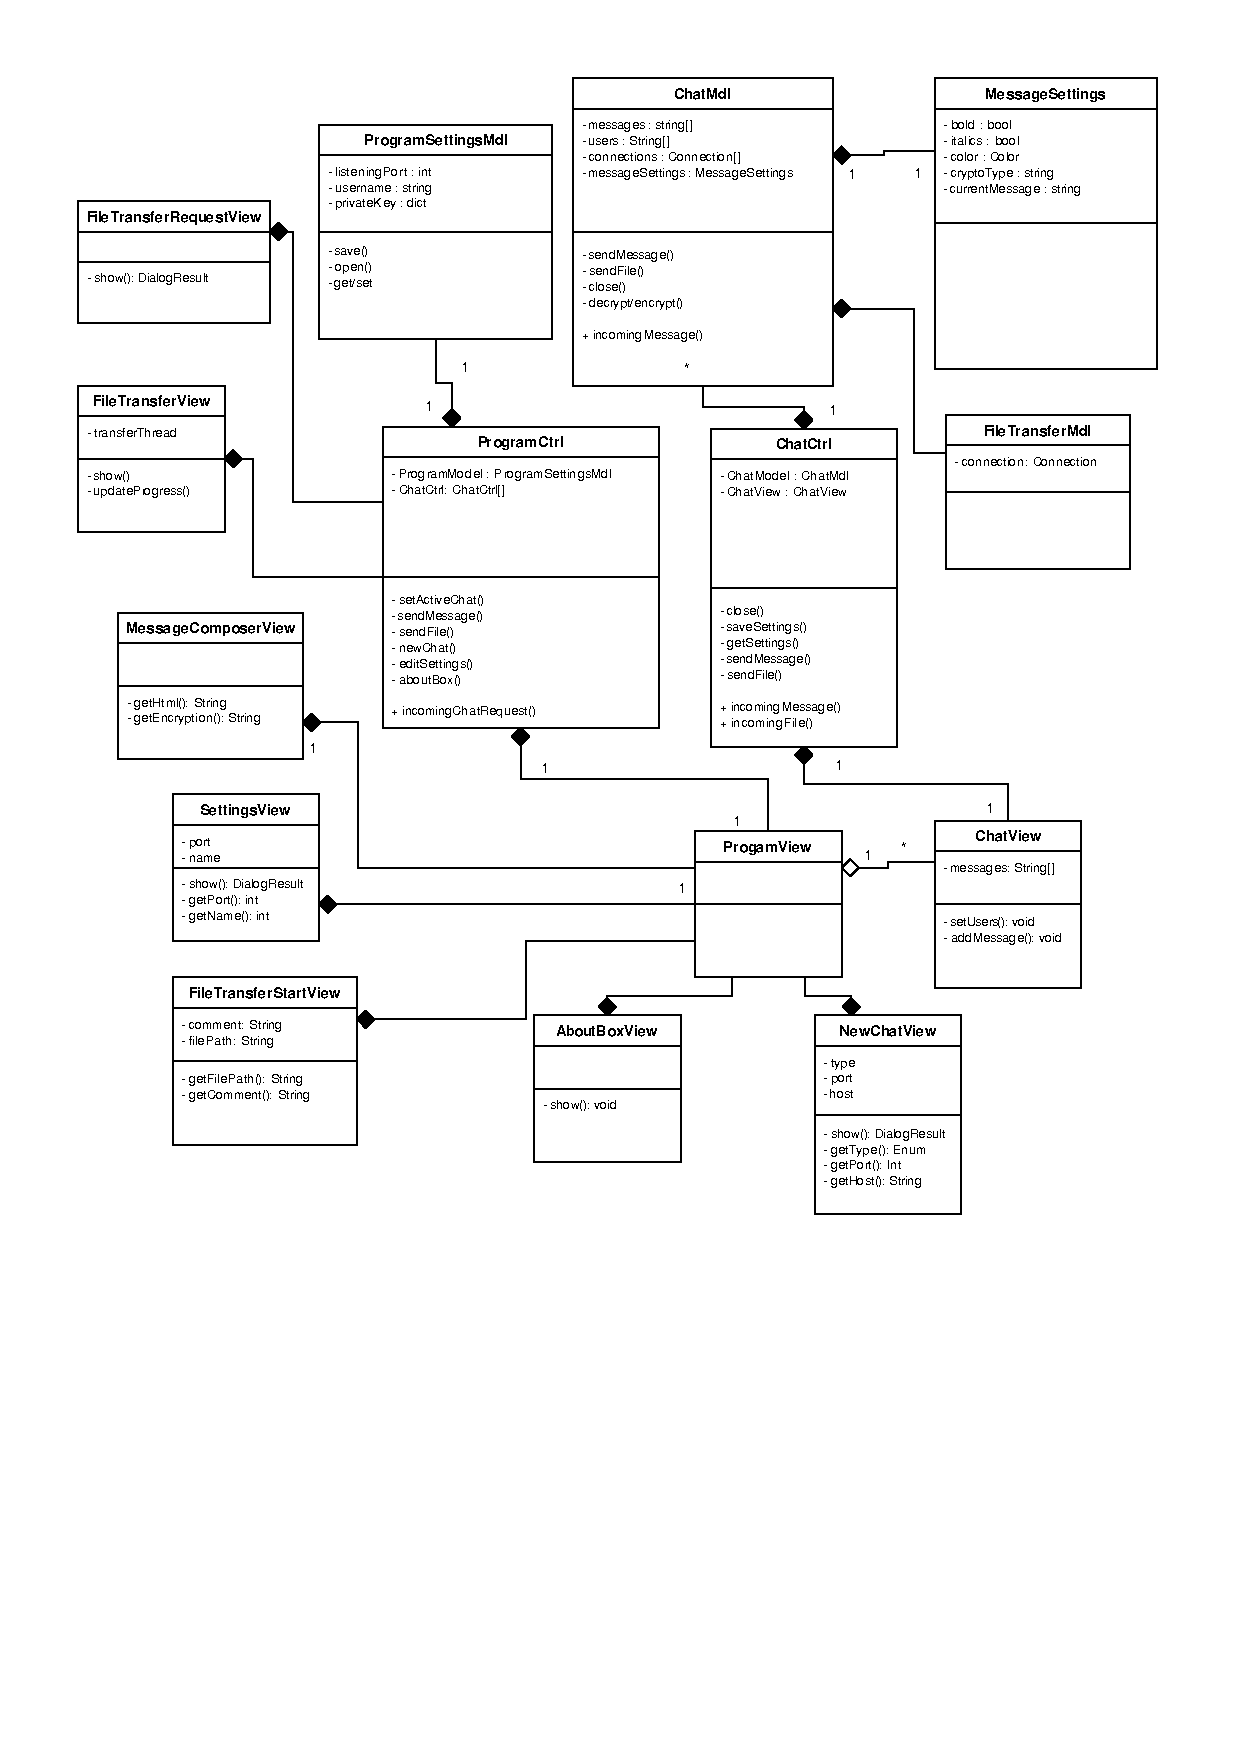
\includegraphics[clip=true, trim=0in 3.5in 0in 0in, width=1.4\textwidth]{../resources/uml.pdf}}
  %\label{fig:key}
\end{figure}

\section{Kontrollflöden}

Nedan beskrivs hur kontrollen flödar mellan klasserna under de olika användningsfallen.

\subsection{Ändra inställningar}

Användaren trycker på Edit $\rightarrow$ Settings. \emph{ProgramView} skapar ett \emph{SettingsView}-objekt och visar det. När användaren stänger dialogrutan kontrolleras om denne sparade och skickar i så fall resultatet till \emph{ProgramCtrl} som uppdaterar \emph{ProgramSettingsMdl}.

\subsection{Ansluta till chat}

Användaren trycker på File $\rightarrow$ New chat. \emph{ProgramView} skapar ett \emph{NewChatView}-objekt och tittar sedan på resultaten. Detta skickas till \emph{ProgramCtrl} som skapar ett \emph{ChatView}-objekt som i sin tur skapar ett \emph{ChatCtrl}-objekt som i sin tur skapar ett \emph{ChatMdl}-objekt. Detta ansluter till värden och börjar kommunicera. \emph{ChatView}-objektet läggs till \emph{ProgramView}-objektet.

\subsection{Ta emot inkommande anslutning}

Programmet får en ny anslutning i \emph{ProgramCtrl}. Den frågar användaren om den vill acceptera anslutningen och skapar i så fall en ny chatt på samma sätt som i förgående avsnitt.

\subsection{Skapa gruppchat}

Användaren trycker på File $\rightarrow$ New chat. Precis som tidigare så skapar \emph{ProgramView} en dialogruta vars resultat skickas till \emph{ProgramCtrl} som skapar en ny chat som tidigare men som lyssnar på en ny port för anslutningar som sedan kan läggas till i \emph{ChatMdl}-objektet.

\subsection{Skicka fil}

Användaren trycker på Send File. \emph{ProgramView} skapar ett \emph{FileTransferStartView}-objekt vars resultat skickas via \emph{ChatView} och \emph{ChatCtrl} till \emph{ChatMdl} som skickar ett meddelande till motparten om filöverföring.

\subsection{Ta emot fil}

\emph{ChatMdl} tar emot ett meddelande om filöverföring vilket skickas till \emph{ProgramCtrl} som, genom ett \emph{FileTransferRequestView}-objekt frågar användaren om den vill ta emot filen. Om ja skickas ett meddelande till avsändaren som öppnar en ny anslutning för filen. Detta sparas i ett \emph{FileTransferMdl}. Både avsändare och mottagare skapar ett \emph{FileTransferView}-objekt som övervakar filöverföringens status.

\end{document}
